\documentclass[twoside]{book}

% Packages required by doxygen
\usepackage{fixltx2e}
\usepackage{calc}
\usepackage{doxygen}
\usepackage{graphicx}
\usepackage[utf8]{inputenc}
\usepackage{makeidx}
\usepackage{multicol}
\usepackage{multirow}
\PassOptionsToPackage{warn}{textcomp}
\usepackage{textcomp}
\usepackage[nointegrals]{wasysym}
\usepackage[table]{xcolor}

% NLS support packages
\usepackage[french]{babel}

% Font selection
\usepackage[T1]{fontenc}
\usepackage{mathptmx}
\usepackage[scaled=.90]{helvet}
\usepackage{courier}
\usepackage{amssymb}
\usepackage{sectsty}
\renewcommand{\familydefault}{\sfdefault}
\allsectionsfont{%
  \fontseries{bc}\selectfont%
  \color{darkgray}%
}
\renewcommand{\DoxyLabelFont}{%
  \fontseries{bc}\selectfont%
  \color{darkgray}%
}
\newcommand{\+}{\discretionary{\mbox{\scriptsize$\hookleftarrow$}}{}{}}

% Page & text layout
\usepackage{geometry}
\geometry{%
  a4paper,%
  top=2.5cm,%
  bottom=2.5cm,%
  left=2.5cm,%
  right=2.5cm%
}
\tolerance=750
\hfuzz=15pt
\hbadness=750
\setlength{\emergencystretch}{15pt}
\setlength{\parindent}{0cm}
\setlength{\parskip}{0.2cm}
\makeatletter
\renewcommand{\paragraph}{%
  \@startsection{paragraph}{4}{0ex}{-1.0ex}{1.0ex}{%
    \normalfont\normalsize\bfseries\SS@parafont%
  }%
}
\renewcommand{\subparagraph}{%
  \@startsection{subparagraph}{5}{0ex}{-1.0ex}{1.0ex}{%
    \normalfont\normalsize\bfseries\SS@subparafont%
  }%
}
\makeatother

% Headers & footers
\usepackage{fancyhdr}
\pagestyle{fancyplain}
\fancyhead[LE]{\fancyplain{}{\bfseries\thepage}}
\fancyhead[CE]{\fancyplain{}{}}
\fancyhead[RE]{\fancyplain{}{\bfseries\leftmark}}
\fancyhead[LO]{\fancyplain{}{\bfseries\rightmark}}
\fancyhead[CO]{\fancyplain{}{}}
\fancyhead[RO]{\fancyplain{}{\bfseries\thepage}}
\fancyfoot[LE]{\fancyplain{}{}}
\fancyfoot[CE]{\fancyplain{}{}}
\fancyfoot[RE]{\fancyplain{}{\bfseries\scriptsize Généré le Mercredi 4 Avril 2018 15\+:14\+:21 pour P\+R\+O\+J\+E\+T P\+I\+C\+R\+O\+S\+S par Doxygen }}
\fancyfoot[LO]{\fancyplain{}{\bfseries\scriptsize Généré le Mercredi 4 Avril 2018 15\+:14\+:21 pour P\+R\+O\+J\+E\+T P\+I\+C\+R\+O\+S\+S par Doxygen }}
\fancyfoot[CO]{\fancyplain{}{}}
\fancyfoot[RO]{\fancyplain{}{}}
\renewcommand{\footrulewidth}{0.4pt}
\renewcommand{\chaptermark}[1]{%
  \markboth{#1}{}%
}
\renewcommand{\sectionmark}[1]{%
  \markright{\thesection\ #1}%
}

% Indices & bibliography
\usepackage{natbib}
\usepackage[titles]{tocloft}
\setcounter{tocdepth}{3}
\setcounter{secnumdepth}{5}
\makeindex

% Hyperlinks (required, but should be loaded last)
\usepackage{ifpdf}
\ifpdf
  \usepackage[pdftex,pagebackref=true]{hyperref}
\else
  \usepackage[ps2pdf,pagebackref=true]{hyperref}
\fi
\hypersetup{%
  colorlinks=true,%
  linkcolor=blue,%
  citecolor=blue,%
  unicode%
}

% Custom commands
\newcommand{\clearemptydoublepage}{%
  \newpage{\pagestyle{empty}\cleardoublepage}%
}


%===== C O N T E N T S =====

\begin{document}

% Titlepage & ToC
\hypersetup{pageanchor=false,
             bookmarks=true,
             bookmarksnumbered=true,
             pdfencoding=unicode
            }
\pagenumbering{roman}
\begin{titlepage}
\vspace*{7cm}
\begin{center}%
{\Large P\+R\+O\+J\+E\+T P\+I\+C\+R\+O\+S\+S }\\
\vspace*{1cm}
{\large Généré par Doxygen 1.8.8}\\
\vspace*{0.5cm}
{\small Mercredi 4 Avril 2018 15:14:21}\\
\end{center}
\end{titlepage}
\clearemptydoublepage
\tableofcontents
\clearemptydoublepage
\pagenumbering{arabic}
\hypersetup{pageanchor=true}

%--- Begin generated contents ---
\chapter{Projet logiciel du semestre 4}
\label{md_README}
\hypertarget{md_README}{}
Membres du groupe \+: \begin{DoxyVerb}* KAJAK Rémi
* KINZI Erick
* MAROUF Taous
* NOUVELIERE Benjamin
\end{DoxyVerb}


Programme développé \+: Picross Description \+:

Le Picross est un jeu de réflexion. Une grille de taille fixe contient N cases vides. Selon les nombres indiqués sur les côtés gauche et haut), le joueur doit cocher les bnnes cases afin de compléter correctement cette grille. Le remplissage des cases en fonction des nombres dépend de deux règles \+: \begin{DoxyVerb}* Un nombre indique un groupe de cases remplies et adjacentes sur une ligne ou une colonne. Il ne peut pas y en avoir plus ou moins que ce nombre.
* Chaque nombre correspond à un groupe de cases, aussi bien horizontalement que verticalement. Chaque groupe est séparé par un espace d'au moins une case vide.
\end{DoxyVerb}


Généralement, un dessin (ou un motif, du moins) se forme au fur et mesure que la grille est complétée. Cela aide aussi le joueur à déterminer la forme finale ainsi que le placement des cases restantes.

\section*{Instructions pour les démonstrations}

Vous trouverez plusieurs exécutables présents à la racine du répertoire. Les fichiers \char`\"{}demo\textbackslash{}\+\_\+cases\char`\"{} et \char`\"{}demo\textbackslash{}\+\_\+generation\textbackslash{}\+\_\+v1\char`\"{} sont des tests unitaires des fichiers éponymes. Pour les re-\/générer, exécutez les makefiles \char`\"{}makefile\textbackslash{}\+\_\+\+Case\char`\"{} et \char`\"{}makefile\textbackslash{}\+\_\+gen\char`\"{} ; attention avec ce dernier \+: comme \char`\"{}generation.\+c\char`\"{} possède deux versions différentes pour la génération de données, veillez à (dé)commenter les bonnes sections dans le main du fichier.

La commande à utiliser est \char`\"{}make -\/f $<$makefile\textbackslash{}\+\_\+nom$>$\char`\"{}.

L'exécutable \char`\"{}demo\textbackslash{}\+\_\+terminal\char`\"{} permet de jouer à la version en mode console du Picross. Pour re-\/générer l'exécutable, appliquez la commande cité précédemment au fichier \char`\"{}makefile\textbackslash{}\+\_\+terminal\char`\"{}.

Pour générer l'exécutable de l'interface graphique, voici les commandes à entrer dans le terminal \+:


\begin{DoxyItemize}
\item gcc picross\+\_\+sdl.\+c sdl2-\/config --cflags --libs -\/l\+S\+D\+L2\+\_\+ttf
\item ./a.out
\end{DoxyItemize}

\section*{Explications du Picross en mode terminal}

Au lancement du jeu, la fenêtre du terminal est nettoyée et la partie se lance automatiquement. Dans cette version, les cases peuvent prendre trois états \+:


\begin{DoxyItemize}
\item 0 -\/$>$ Blanche =$>$ Case vide
\item 1 -\/$>$ Noire =$>$ Case cochée
\item 2 -\/$>$ Croix =$>$ Case assurément vide (pour permettre les suppositions)
\end{DoxyItemize}

Vous devez résoudre les six puzzles proposés dans cette première version (sans solveur) \+:


\begin{DoxyItemize}
\item À chaque tour, le jeu vous demande deux coordonnées x et y, respectivement pour une ligne et une colonne ; =$>$ En cas d'erreur de saisie pour l'une ou pour l'autre, le programme bloquera le tour jusqu'à ce qu'elles soient correctes.
\item Une fois vos choix effectués, vous pouvez valider votre grille avec les coordonnées -\/1 et -\/1 ;
\item Le programme vous renverra soit un message de félicitation pour avoir résolu le puzzle, soit un message d'erreur avec le nombre de mauvaises cases cochées ; =$>$ Dans les deux cas, vous pouvez choisir de quitter la partie (et donc le programme) ou de continuer à jouer.
\item Le jeu se termine automatiquement si vous résolvez tous les puzzles ! 
\end{DoxyItemize}
\chapter{Index des classes}
\section{Liste des classes}
Liste des classes, structures, unions et interfaces avec une brève description \+:\begin{DoxyCompactList}
\item\contentsline{section}{\hyperlink{structcocher}{cocher} }{\pageref{structcocher}}{}
\end{DoxyCompactList}

\chapter{Index des fichiers}
\section{Liste des fichiers}
Liste de tous les fichiers documentés avec une brève description \+:\begin{DoxyCompactList}
\item\contentsline{section}{\hyperlink{Case_8c}{Case.\+c} \\*Représentation des cases }{\pageref{Case_8c}}{}
\item\contentsline{section}{\hyperlink{Case_8h}{Case.\+h} \\*Contient les définitions des structures enum et des fonctions de \char`\"{}\+Case.\+c\char`\"{} }{\pageref{Case_8h}}{}
\item\contentsline{section}{\hyperlink{generation_8c}{generation.\+c} \\*Fichier ayant servi à l'élaboration des différentes fonctions de génération des trois matrices principales }{\pageref{generation_8c}}{}
\item\contentsline{section}{\hyperlink{generation_8h}{generation.\+h} \\*Fichier contenant les définitions des fonctions de \char`\"{}generation.\+c\char`\"{}. Fait appel à \char`\"{}\+Case.\+h\char`\"{} pour obtenir les définitions et les structures de \char`\"{}\+Case.\+c\char`\"{} }{\pageref{generation_8h}}{}
\item\contentsline{section}{\hyperlink{terminal_8c}{terminal.\+c} \\*Fichier permettant de jouer une partie de Picross à partir d'un terminal de commande }{\pageref{terminal_8c}}{}
\end{DoxyCompactList}

\chapter{Documentation des classes}
\hypertarget{structcocher}{\section{Référence de la structure cocher}
\label{structcocher}\index{cocher@{cocher}}
}


Graphe de collaboration de cocher\+:\nopagebreak
\begin{figure}[H]
\begin{center}
\leavevmode
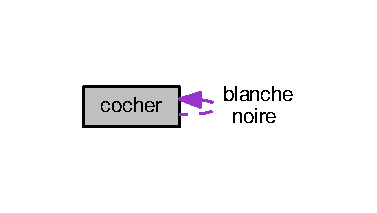
\includegraphics[width=181pt]{structcocher__coll__graph}
\end{center}
\end{figure}
\subsection*{Attributs publics}
\begin{DoxyCompactItemize}
\item 
\hypertarget{structcocher_a1bc69d5a9e615b8ace629bdc3794e0ef}{int {\bfseries croix}}\label{structcocher_a1bc69d5a9e615b8ace629bdc3794e0ef}

\item 
\hypertarget{structcocher_a09aea59afcce00c90dbe2911ae437452}{struct \hyperlink{structcocher}{cocher} $\ast$ {\bfseries noire}}\label{structcocher_a09aea59afcce00c90dbe2911ae437452}

\item 
\hypertarget{structcocher_a445ec08e89d9ad03ac07ec3b07f6153f}{struct \hyperlink{structcocher}{cocher} $\ast$ {\bfseries blanche}}\label{structcocher_a445ec08e89d9ad03ac07ec3b07f6153f}

\end{DoxyCompactItemize}


La documentation de cette structure a été générée à partir des fichiers suivants \+:\begin{DoxyCompactItemize}
\item 
case\+\_\+.\+c\item 
case\+\_\+.\+h\end{DoxyCompactItemize}

\chapter{Documentation des fichiers}
\hypertarget{generation_8c}{\section{Référence du fichier generation.\+c}
\label{generation_8c}\index{generation.\+c@{generation.\+c}}
}


Fichier ayant servi à l'élaboration des différentes fonctions de génération des trois matrices principales.  


{\ttfamily \#include $<$stdio.\+h$>$}\\*
{\ttfamily \#include $<$stdlib.\+h$>$}\\*
{\ttfamily \#include $<$string.\+h$>$}\\*
{\ttfamily \#include \char`\"{}generation.\+h\char`\"{}}\\*
Graphe des dépendances par inclusion de generation.\+c\+:\nopagebreak
\begin{figure}[H]
\begin{center}
\leavevmode
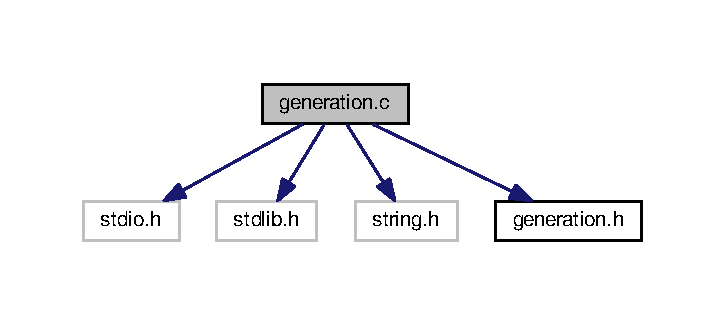
\includegraphics[width=348pt]{generation_8c__incl}
\end{center}
\end{figure}
\subsection*{Fonctions}
\begin{DoxyCompactItemize}
\item 
int $\ast$ \hyperlink{generation_8c_a75844feaf083b06c8757f2ade3239305}{init\+\_\+matrice\+\_\+periph} (t\+\_\+difficulte taille\+\_\+max)
\begin{DoxyCompactList}\small\item\em Initialise une matrice avec des 0. \end{DoxyCompactList}\item 
void \hyperlink{generation_8c_aecb99c4032546fdf1fae4a3ab2ed8b80}{afficher\+\_\+matrice} (int $\ast$mat, t\+\_\+difficulte taille, char cle)
\begin{DoxyCompactList}\small\item\em Affiche une matrice reçue en paramètre selon un modèle prédéfini. \end{DoxyCompactList}\item 
void \hyperlink{generation_8c_a021a69096e7e1b7e11c2e21d360faa64}{lecture\+\_\+fic\+\_\+v1} (char $\ast$nom\+\_\+fic, int puzzle, t\+\_\+couleurs $\ast$soluce, t\+\_\+difficulte taille)
\begin{DoxyCompactList}\small\item\em Lit un fichier avec un format spécifique et remplit une matrice solution (première version du jeu). \end{DoxyCompactList}\item 
void \hyperlink{generation_8c_a901f56ea1ee28707a99d258553a4efca}{gen\+\_\+peripheriques} (t\+\_\+couleurs $\ast$soluce, int $\ast$colonnes, int $\ast$lignes, t\+\_\+difficulte taille)
\begin{DoxyCompactList}\small\item\em Lit la matrice solution et génère les nombres correspondant aux groupes de cases pleines de chaque rangée dans les bonnes matrices périphériques. \end{DoxyCompactList}\end{DoxyCompactItemize}


\subsection{Description détaillée}
Fichier ayant servi à l'élaboration des différentes fonctions de génération des trois matrices principales. 

\begin{DoxyAuthor}{Auteur}
K\+A\+J\+A\+K Rémi 
\end{DoxyAuthor}
\begin{DoxyVersion}{Version}
1.\+2 
\end{DoxyVersion}
\begin{DoxyDate}{Date}
07/04/2018 
\end{DoxyDate}


\subsection{Documentation des fonctions}
\hypertarget{generation_8c_aecb99c4032546fdf1fae4a3ab2ed8b80}{\index{generation.\+c@{generation.\+c}!afficher\+\_\+matrice@{afficher\+\_\+matrice}}
\index{afficher\+\_\+matrice@{afficher\+\_\+matrice}!generation.\+c@{generation.\+c}}
\subsubsection[{afficher\+\_\+matrice}]{\setlength{\rightskip}{0pt plus 5cm}afficher\+\_\+matrice (
\begin{DoxyParamCaption}
\item[{int $\ast$}]{mat, }
\item[{t\+\_\+difficulte}]{taille, }
\item[{char}]{cle}
\end{DoxyParamCaption}
)}}\label{generation_8c_aecb99c4032546fdf1fae4a3ab2ed8b80}


Affiche une matrice reçue en paramètre selon un modèle prédéfini. 


\begin{DoxyParams}{Paramètres}
{\em mat} & Une matrice de taille fixe \\
\hline
{\em taille} & La taille de la matrice indiquée par le niveau de difficulté \\
\hline
{\em cle} & Un caractère qui définit le mode d'affichage \+: \char`\"{}\+C\char`\"{} pour afficher horizontalement les nombres de la matrice périphérique des colonnes et \char`\"{}\+L\char`\"{} pour afficher verticalement les nombres de la matrice périphérique des lignes\\
\hline
\end{DoxyParams}
\begin{DoxyReturn}{Renvoie}
Ne retourne aucun résultat 
\end{DoxyReturn}
\hypertarget{generation_8c_a901f56ea1ee28707a99d258553a4efca}{\index{generation.\+c@{generation.\+c}!gen\+\_\+peripheriques@{gen\+\_\+peripheriques}}
\index{gen\+\_\+peripheriques@{gen\+\_\+peripheriques}!generation.\+c@{generation.\+c}}
\subsubsection[{gen\+\_\+peripheriques}]{\setlength{\rightskip}{0pt plus 5cm}gen\+\_\+peripheriques (
\begin{DoxyParamCaption}
\item[{t\+\_\+couleurs $\ast$}]{soluce, }
\item[{int $\ast$}]{colonnes, }
\item[{int $\ast$}]{lignes, }
\item[{t\+\_\+difficulte}]{taille}
\end{DoxyParamCaption}
)}}\label{generation_8c_a901f56ea1ee28707a99d258553a4efca}


Lit la matrice solution et génère les nombres correspondant aux groupes de cases pleines de chaque rangée dans les bonnes matrices périphériques. 


\begin{DoxyParams}{Paramètres}
{\em soluce} & La matrice solution de type enum \\
\hline
{\em colonnes} & La matrice périphérique des colonnes \\
\hline
{\em lignes} & La matrice périphérique des lignes \\
\hline
{\em taille} & La taille des matrices renseignées\\
\hline
\end{DoxyParams}
\begin{DoxyReturn}{Renvoie}
Ne retourne aucun résultat 
\end{DoxyReturn}
\hypertarget{generation_8c_a75844feaf083b06c8757f2ade3239305}{\index{generation.\+c@{generation.\+c}!init\+\_\+matrice\+\_\+periph@{init\+\_\+matrice\+\_\+periph}}
\index{init\+\_\+matrice\+\_\+periph@{init\+\_\+matrice\+\_\+periph}!generation.\+c@{generation.\+c}}
\subsubsection[{init\+\_\+matrice\+\_\+periph}]{\setlength{\rightskip}{0pt plus 5cm}init\+\_\+matrice\+\_\+periph (
\begin{DoxyParamCaption}
\item[{t\+\_\+difficulte}]{taille\+\_\+max}
\end{DoxyParamCaption}
)}}\label{generation_8c_a75844feaf083b06c8757f2ade3239305}


Initialise une matrice avec des 0. 


\begin{DoxyParams}{Paramètres}
{\em taille\+\_\+max} & La taille maximum de la matrice à initialiser\\
\hline
\end{DoxyParams}
\begin{DoxyReturn}{Renvoie}
Une matrice de type int allouée dynamiquement 
\end{DoxyReturn}
\hypertarget{generation_8c_a021a69096e7e1b7e11c2e21d360faa64}{\index{generation.\+c@{generation.\+c}!lecture\+\_\+fic\+\_\+v1@{lecture\+\_\+fic\+\_\+v1}}
\index{lecture\+\_\+fic\+\_\+v1@{lecture\+\_\+fic\+\_\+v1}!generation.\+c@{generation.\+c}}
\subsubsection[{lecture\+\_\+fic\+\_\+v1}]{\setlength{\rightskip}{0pt plus 5cm}lecture\+\_\+fic\+\_\+v1 (
\begin{DoxyParamCaption}
\item[{char $\ast$}]{nom\+\_\+fic, }
\item[{int}]{puzzle, }
\item[{t\+\_\+couleurs $\ast$}]{soluce, }
\item[{t\+\_\+difficulte}]{taille}
\end{DoxyParamCaption}
)}}\label{generation_8c_a021a69096e7e1b7e11c2e21d360faa64}


Lit un fichier avec un format spécifique et remplit une matrice solution (première version du jeu). 


\begin{DoxyParams}{Paramètres}
{\em nom\+\_\+fic} & Nom du fichier texte à analyser \\
\hline
{\em puzzle} & Numéro du puzzle à trouver dans le fichier \\
\hline
{\em soluce} & La matrice solution de type enum \\
\hline
{\em taille} & La taille de la matrice renseignée\\
\hline
\end{DoxyParams}
\begin{DoxyReturn}{Renvoie}
Ne retourne aucun résultat 
\end{DoxyReturn}

\hypertarget{terminal_8c}{\section{Référence du fichier terminal.\+c}
\label{terminal_8c}\index{terminal.\+c@{terminal.\+c}}
}


Fichier permettant de jouer une partie de Picross à partir d'un terminal de commande.  


{\ttfamily \#include $<$stdio.\+h$>$}\\*
{\ttfamily \#include $<$stdlib.\+h$>$}\\*
Graphe des dépendances par inclusion de terminal.\+c\+:\nopagebreak
\begin{figure}[H]
\begin{center}
\leavevmode
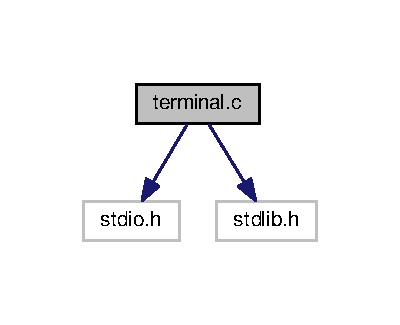
\includegraphics[width=192pt]{terminal_8c__incl}
\end{center}
\end{figure}
\subsection*{Définitions de type}
\begin{DoxyCompactItemize}
\item 
\hypertarget{terminal_8c_a94756a97e8544e427ec192d822e8d18d}{typedef enum couleurs {\bfseries t\+\_\+couleurs}}\label{terminal_8c_a94756a97e8544e427ec192d822e8d18d}

\item 
\hypertarget{terminal_8c_ac44c29a89ad2278798bb0c02e4282afb}{typedef enum difficulte {\bfseries t\+\_\+difficulte}}\label{terminal_8c_ac44c29a89ad2278798bb0c02e4282afb}

\end{DoxyCompactItemize}
\subsection*{Énumérations}
\begin{DoxyCompactItemize}
\item 
\hypertarget{terminal_8c_ae8772b89c073fcb61b7a2482b1192b3e}{enum {\bfseries couleurs} \{ \\*
{\bfseries Blanche}, 
{\bfseries Noire}, 
{\bfseries Croix}, 
{\bfseries Blanche}, 
\\*
{\bfseries Noire}, 
{\bfseries Croix}, 
{\bfseries Blanche}, 
{\bfseries Noire}, 
\\*
{\bfseries Croix}
 \}}\label{terminal_8c_ae8772b89c073fcb61b7a2482b1192b3e}

\item 
\hypertarget{terminal_8c_a35aa2d55b501700469097f04b7962297}{enum {\bfseries difficulte} \{ \\*
{\bfseries facile} = 3, 
{\bfseries normal}, 
{\bfseries difficile}, 
{\bfseries expert} = 10, 
\\*
{\bfseries facile} =3, 
{\bfseries normal} =5, 
{\bfseries difficile} =7, 
{\bfseries expert} =10, 
\\*
{\bfseries facile} =3, 
{\bfseries normal} =5, 
{\bfseries difficile} =7, 
{\bfseries expert} =10
 \}}\label{terminal_8c_a35aa2d55b501700469097f04b7962297}

\end{DoxyCompactItemize}
\subsection*{Fonctions}
\begin{DoxyCompactItemize}
\item 
\hypertarget{terminal_8c_ac848923fd27c9cbcb10c985e1b11d1a9}{t\+\_\+couleurs $\ast$ {\bfseries init\+\_\+matrice\+\_\+prin} (t\+\_\+difficulte dim\+\_\+mat)}\label{terminal_8c_ac848923fd27c9cbcb10c985e1b11d1a9}

\item 
\hypertarget{terminal_8c_a8422b2d48cb1567687a27006431cde21}{int $\ast$ {\bfseries init\+\_\+matrice\+\_\+peri} (t\+\_\+difficulte dim\+\_\+mat)}\label{terminal_8c_a8422b2d48cb1567687a27006431cde21}

\item 
\hypertarget{terminal_8c_a9a72073891fc1ec027db352bc45f1628}{void {\bfseries detruire\+\_\+matrice\+\_\+peri} (int $\ast$mat)}\label{terminal_8c_a9a72073891fc1ec027db352bc45f1628}

\item 
\hypertarget{terminal_8c_a7b957b79fcc220384d87524b4b85c435}{void {\bfseries detruire\+\_\+matrice\+\_\+prin} (t\+\_\+couleurs $\ast$mat)}\label{terminal_8c_a7b957b79fcc220384d87524b4b85c435}

\item 
\hypertarget{terminal_8c_a49722fa6c282bc49add2ceeb59f88104}{void {\bfseries afficher\+\_\+haut} (int $\ast$mat\+\_\+hori, t\+\_\+difficulte dim\+\_\+mat)}\label{terminal_8c_a49722fa6c282bc49add2ceeb59f88104}

\item 
\hypertarget{terminal_8c_aa3e98d3cfbf4db36ba1afb4a1bf5a30c}{void {\bfseries afficher\+\_\+bas} (int $\ast$mat\+\_\+verti, t\+\_\+couleurs $\ast$mat\+\_\+prin, t\+\_\+difficulte dim\+\_\+mat)}\label{terminal_8c_aa3e98d3cfbf4db36ba1afb4a1bf5a30c}

\item 
\hypertarget{terminal_8c_ab1e6ec88ae60e83eab1cc131a79ad000}{void {\bfseries affichage\+\_\+jeu} (int $\ast$mat\+\_\+hori, int $\ast$mat\+\_\+verti, t\+\_\+couleurs $\ast$mat\+\_\+prin, t\+\_\+difficulte dim\+\_\+mat)}\label{terminal_8c_ab1e6ec88ae60e83eab1cc131a79ad000}

\item 
void \hyperlink{terminal_8c_a7731ac5d32100449a8e2480d599a70cb}{changer\+Etat} (t\+\_\+couleurs $\ast$mat\+\_\+prin, t\+\_\+difficulte dim\+\_\+mat, int x, int y)
\begin{DoxyCompactList}\small\item\em Fonction qui permet de changer l'état de la case. \end{DoxyCompactList}\item 
int \hyperlink{terminal_8c_aaf69df6150ddf60905ed92f6b47447aa}{saisir\+\_\+coord} (t\+\_\+couleurs $\ast$mat\+\_\+prin, t\+\_\+difficulte dim\+\_\+mat)
\begin{DoxyCompactList}\small\item\em Fonction qui permet à l'utilisateur d'entrer des coordonnées. \end{DoxyCompactList}\item 
void \hyperlink{terminal_8c_a3e9c8b3fe82c9af0c1dea882df430528}{lecture\+\_\+fic\+\_\+v1} (char $\ast$nom\+\_\+fic, int puzzle, t\+\_\+couleurs $\ast$soluce, t\+\_\+difficulte taille)
\begin{DoxyCompactList}\small\item\em Lit un fichier avec un format spécifique et remplit une matrice solution (première version du jeu). \end{DoxyCompactList}\item 
void \hyperlink{terminal_8c_a1126745af00395f3f057e7f1c51b0164}{gen\+\_\+peripheriques} (t\+\_\+couleurs $\ast$soluce, int $\ast$colonnes, int $\ast$lignes, t\+\_\+difficulte taille)
\begin{DoxyCompactList}\small\item\em Lit la matrice solution et génère les nombres correspondant aux groupes de cases pleines de chaque rangée dans les bonnes matrices périphériques. \end{DoxyCompactList}\item 
\hypertarget{terminal_8c_a8a74374a913d4fb5d06612ed4992170a}{int {\bfseries verif\+\_\+soluce} (t\+\_\+couleurs $\ast$mat\+\_\+prin, t\+\_\+couleurs $\ast$mat\+\_\+soluce, int dim\+\_\+mat)}\label{terminal_8c_a8a74374a913d4fb5d06612ed4992170a}

\item 
\hypertarget{terminal_8c_a840291bc02cba5474a4cb46a9b9566fe}{int {\bfseries main} (void)}\label{terminal_8c_a840291bc02cba5474a4cb46a9b9566fe}

\end{DoxyCompactItemize}


\subsection{Description détaillée}
Fichier permettant de jouer une partie de Picross à partir d'un terminal de commande. 

\begin{DoxyAuthor}{Auteur}
K\+A\+J\+A\+K Rémi 
\end{DoxyAuthor}
\begin{DoxyVersion}{Version}
1.\+0 
\end{DoxyVersion}
\begin{DoxyDate}{Date}
03/04/2018 
\end{DoxyDate}


\subsection{Documentation des fonctions}
\hypertarget{terminal_8c_a7731ac5d32100449a8e2480d599a70cb}{\index{terminal.\+c@{terminal.\+c}!changer\+Etat@{changer\+Etat}}
\index{changer\+Etat@{changer\+Etat}!terminal.\+c@{terminal.\+c}}
\subsubsection[{changer\+Etat}]{\setlength{\rightskip}{0pt plus 5cm}void changer\+Etat (
\begin{DoxyParamCaption}
\item[{t\+\_\+couleurs $\ast$}]{mat\+\_\+prin, }
\item[{t\+\_\+difficulte}]{dim\+\_\+mat, }
\item[{int}]{x, }
\item[{int}]{y}
\end{DoxyParamCaption}
)}}\label{terminal_8c_a7731ac5d32100449a8e2480d599a70cb}


Fonction qui permet de changer l'état de la case. 


\begin{DoxyParams}{Paramètres}
{\em mat} & La matrice qui représente la grille \\
\hline
{\em taille} & La taille de la matrice renseignée \\
\hline
{\em x} & Une coordonnée renseignant l'abscisse d'une matrice \\
\hline
{\em y} & Une coordonnée renseignant l'ordonnée d'une matrice\\
\hline
\end{DoxyParams}
\begin{DoxyReturn}{Renvoie}
Ne retourne aucune valeur 
\end{DoxyReturn}
\hypertarget{terminal_8c_a1126745af00395f3f057e7f1c51b0164}{\index{terminal.\+c@{terminal.\+c}!gen\+\_\+peripheriques@{gen\+\_\+peripheriques}}
\index{gen\+\_\+peripheriques@{gen\+\_\+peripheriques}!terminal.\+c@{terminal.\+c}}
\subsubsection[{gen\+\_\+peripheriques}]{\setlength{\rightskip}{0pt plus 5cm}void gen\+\_\+peripheriques (
\begin{DoxyParamCaption}
\item[{t\+\_\+couleurs $\ast$}]{soluce, }
\item[{int $\ast$}]{colonnes, }
\item[{int $\ast$}]{lignes, }
\item[{t\+\_\+difficulte}]{taille}
\end{DoxyParamCaption}
)}}\label{terminal_8c_a1126745af00395f3f057e7f1c51b0164}


Lit la matrice solution et génère les nombres correspondant aux groupes de cases pleines de chaque rangée dans les bonnes matrices périphériques. 


\begin{DoxyParams}{Paramètres}
{\em soluce} & La matrice solution de type enum \\
\hline
{\em colonnes} & La matrice périphérique des colonnes \\
\hline
{\em lignes} & La matrice périphérique des lignes \\
\hline
{\em taille} & La taille des matrices renseignées\\
\hline
\end{DoxyParams}
\begin{DoxyReturn}{Renvoie}
Ne retourne aucun résultat 
\end{DoxyReturn}
\hypertarget{terminal_8c_a3e9c8b3fe82c9af0c1dea882df430528}{\index{terminal.\+c@{terminal.\+c}!lecture\+\_\+fic\+\_\+v1@{lecture\+\_\+fic\+\_\+v1}}
\index{lecture\+\_\+fic\+\_\+v1@{lecture\+\_\+fic\+\_\+v1}!terminal.\+c@{terminal.\+c}}
\subsubsection[{lecture\+\_\+fic\+\_\+v1}]{\setlength{\rightskip}{0pt plus 5cm}void lecture\+\_\+fic\+\_\+v1 (
\begin{DoxyParamCaption}
\item[{char $\ast$}]{nom\+\_\+fic, }
\item[{int}]{puzzle, }
\item[{t\+\_\+couleurs $\ast$}]{soluce, }
\item[{t\+\_\+difficulte}]{taille}
\end{DoxyParamCaption}
)}}\label{terminal_8c_a3e9c8b3fe82c9af0c1dea882df430528}


Lit un fichier avec un format spécifique et remplit une matrice solution (première version du jeu). 


\begin{DoxyParams}{Paramètres}
{\em nom\+\_\+fic} & Nom du fichier texte à analyser \\
\hline
{\em puzzle} & Numéro du puzzle à trouver dans le fichier \\
\hline
{\em soluce} & La matrice solution de type enum \\
\hline
{\em taille} & La taille de la matrice renseignée\\
\hline
\end{DoxyParams}
\begin{DoxyReturn}{Renvoie}
Ne retourne aucun résultat 
\end{DoxyReturn}
\hypertarget{terminal_8c_aaf69df6150ddf60905ed92f6b47447aa}{\index{terminal.\+c@{terminal.\+c}!saisir\+\_\+coord@{saisir\+\_\+coord}}
\index{saisir\+\_\+coord@{saisir\+\_\+coord}!terminal.\+c@{terminal.\+c}}
\subsubsection[{saisir\+\_\+coord}]{\setlength{\rightskip}{0pt plus 5cm}int saisir\+\_\+coord (
\begin{DoxyParamCaption}
\item[{t\+\_\+couleurs $\ast$}]{mat\+\_\+prin, }
\item[{t\+\_\+difficulte}]{dim\+\_\+mat}
\end{DoxyParamCaption}
)}}\label{terminal_8c_aaf69df6150ddf60905ed92f6b47447aa}


Fonction qui permet à l'utilisateur d'entrer des coordonnées. 


\begin{DoxyParams}{Paramètres}
{\em mat} & La matrice de type enum qui représente la grille \\
\hline
{\em taille} & La taille de la matrice renseignée\\
\hline
\end{DoxyParams}
\begin{DoxyReturn}{Renvoie}
Retourne l'état de la sélection, si le joueur souhaite soumettre sa grille à la vérification ou pas 
\end{DoxyReturn}

%--- End generated contents ---

% Index
\newpage
\phantomsection
\addcontentsline{toc}{chapter}{Index}
\printindex

\end{document}
